%\documentclass[12pt,handout]{beamer}
\documentclass{beamer}
\usepackage[ngerman]{babel}
\usepackage[utf8]{inputenc}
\usepackage{amsmath}
\usepackage{amssymb}
\usepackage{listings} 
\usepackage{stmaryrd}
\lstset{language=Python, tabsize=4, showstringspaces=false,basicstyle=\tiny,mathescape=true}
\lstset{literate=%
  {Ö}{{\"O}}1
  {Ä}{{\"A}}1
  {Ü}{{\"U}}1
  {ß}{{\ss}}1
  {ü}{{\"u}}1
  {ä}{{\"a}}1
  {ö}{{\"o}}1
}
\usepackage{mathtools}
\usepackage{ulem}
\usepackage{tikz}

\usetheme{Boadilla}
\mode<presentation>{
\useoutertheme[subsection=false]{miniframes}
\useinnertheme{rectangles}
%\usecolortheme{crane}
}
\parskip 10pt



\begin{document}
\title{Informatik}   
\author{Abstrakte Datentypen - Keller und Schlange} 
\date{}
\frame{\titlepage} 

%---

\begin{frame}[fragile]

ADT Keller  (= Stapel, stack)  

Prinzip LIFO: Last in, First Out

Ein Keller ist eine (ggf. leere) Folge von Elementen zusammen mit einem so genannten
(ggf. undefinierten) Top-Element.  

Schnittstelle des ADT Keller:

\footnotesize
\begin{tabular}{l l l}
 empty & :  & liefert true, falls Keller leer \\
 push & :  &  legt Element auf Keller \\
 top & :   & liefert oberstes Kellerelement\\ 
 pop & :  &  entfernt oberstes Kellerelement \\
\end{tabular}
\end{frame}

%---
\begin{frame}[fragile]
Wie sollen wir verzeigern?

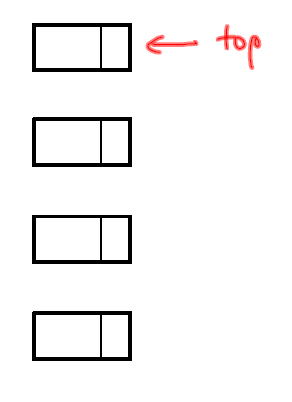
\includegraphics[scale=0.6]{keller1.png} \pause 
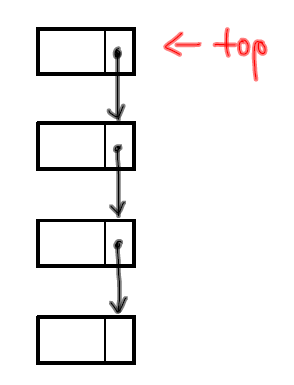
\includegraphics[scale=0.6]{keller2.png}

\end{frame}

%---
\begin{frame}[fragile]
Anwendungsbeispiel: 
Korrektheit der Klammerung mittels Keller bestimmen:

$(((a+b) \cdot c + (a+c) \cdot 2) -3) \cdot 5$     ~~~~~~~~~ korrekt geklammert

$(((a+b) \cdot c + (a+c) \cdot 2)) -3) \cdot 5$   ~~~~~~~~ nicht korrekt geklammert

\end{frame}

\begin{frame}[fragile]
\begin{lstlisting}[mathescape=true]
class Keller:
    def __init__(self):   $\pause$
        self.tp = None

    def empty(self):    $\pause$
        return self.tp is None

    def push(self, x):   $\pause$
        hilf = Eintrag()
        hilf.inhalt = x
        hilf.next = self.tp
        self.tp = hilf

    def top(self):   $\pause$
        if self.empty(): raise RuntimeError("Fehler: Keller ist leer")
        return self.tp.inhalt

    def pop(self):  $\pause$
         if self.empty(): raise RuntimeError("Fehler: Keller ist leer")
         self.tp = self.tp.next
\end{lstlisting}
\end{frame}


\begin{frame}[fragile]

ADT Schlange  

Eine Schlange ist eine (ggf. leere) Folge von Elementen zusammen mit einem so genannten
(ggf. undefinierten) Front-Element.  

Prinzip FIFO: First in, First Out  

Schnittstelle des ADT Schlange:

\footnotesize
\begin{tabular}{l l l}
 empty & : & liefert true, falls Schlange leer \\
 enq & : &  fügt Element hinten ein\\
 front & :  & liefert vorderstes Element\\ 
 deq & : &  entfernt vorderstes Element \\
\end{tabular}

\end{frame}


%---
\begin{frame}[fragile]
Wie sollen wir verzeigern?

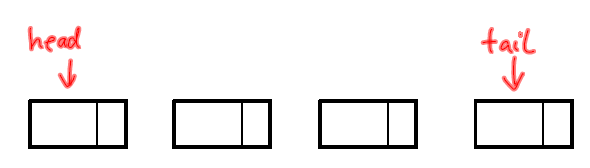
\includegraphics[scale=0.6]{schlange1.png}  \pause 

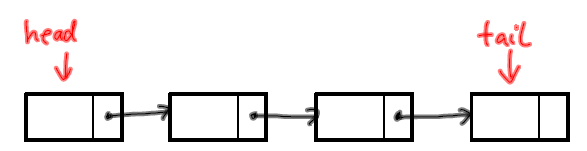
\includegraphics[scale=0.6]{schlange2.png}

\end{frame}


\begin{frame}[fragile]
\begin{lstlisting}[mathescape=true]
class Schlange:
    def __init__(self):   $\pause$
        self.head = None
        self.tail = None

    def empty(self):  $\pause$
        return self.head is None

    def enq(self, x):  $\pause$
        hilf = Eintrag()
        hilf.inhalt = x
        if self.empty():
            self.head = hilf
            self.tail = hilf
        else:
            self.tail.next = hilf
            self.tail = hilf

    def deq(self):  $\pause$
         if self.empty(): raise RuntimeError("Fehler: Schlange ist leer")
         self.head = self.head.next
         if self.head is None:
             self.tail = None

    def front(self):  $\pause$
         if self.empty(): raise RuntimeError("Fehler: Schlange ist leer")
         return self.head.inhalt
\end{lstlisting} 
\end{frame}
\end{document}